\section{Evaluation}
\label{sec:experiments}

We evaluate \ssrov{} through conflicts on observed allocation paths, system cost and a live path control, routing benefit and exposure, and the reachability an adversary gains.

\subsection{Conflicts during Partial ROA Issuance}
\label{sec:eval-conflict-reduction}

\emph{How does \ssrov{} reduce conflicts during partial ROA issuance?} From Table~\ref{tab:visibility-candidates}, 587 endpoint prefixes yield 589 route--origin pairs under 97 aggregate prefixes, because two IPv4 endpoints have two observed origins; matching ROAs are issued atomically per endpoint and cover its complete observed origin set.

Figure~\ref{fig:partial-policy-coverage} reports the mean share of these pairs classified \invalid{} over 1,000 seeded replays, stepping ROA issuance from 0\% to 100\% in 10\% increments and policy coverage from 0\% to 100\% in 20\% increments under randomized, nested selections. \subref{fig:partial-policy-potential} keeps every aggregate ROA active, while \subref{fig:partial-policy-observed} activates sampled aggregate and downstream ROAs jointly, so an observed conflict needs an active aggregate ROA, an absent downstream ROA, and a route that no applicable policy admits.

\begin{figure}[tb]\centering
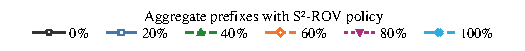
\includegraphics[width=0.9\columnwidth,trim=0 5bp 0 0,clip]{figures/fig_partial_policy_legend}\par
{\captionsetup[subfloat]{farskip=0pt}%
\subfloat[Potential conflicts.]{%
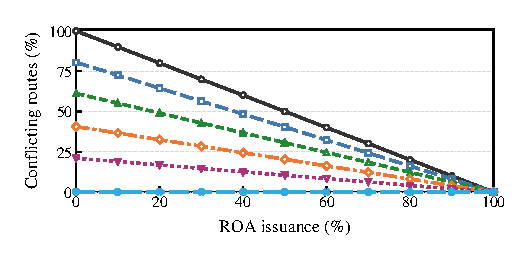
\includegraphics[width=0.9\columnwidth,trim=0 10bp 0 0,clip]{figures/fig_partial_policy_potential}%
\label{fig:partial-policy-potential}}}\par
\subfloat[Observed conflicts.]{%
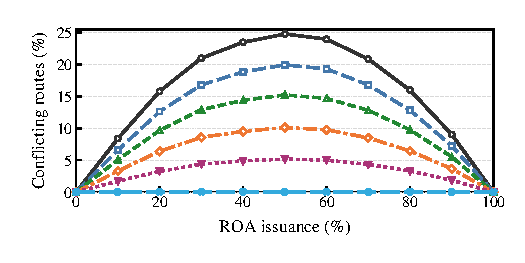
\includegraphics[width=0.9\columnwidth,trim=0 10bp 0 0,clip]{figures/fig_partial_policy_observed}%
\label{fig:partial-policy-observed}}
\subfigmaincaptionskip
\caption{Conflicts during partial ROA issuance.}
\label{fig:partial-policy-coverage}
\end{figure}

At 50\% issuance, conventional ROV leaves mean potential and observed conflict rates of 50.1\% and 24.8\%. Policies on 80\% of the aggregate prefixes lower them to 10.5\% and 5.2\%, relative reductions of 79.1\% in both views; covering all aggregate prefixes leaves 0.1\% and $<0.1\%$ because one observed origin is ineligible, while full downstream issuance makes every route \explicit{}. \ssrov{} therefore lowers both the potential conflicts that aggregate ROAs create and the peak during partial issuance.

\emph{Which aggregate prefixes should be configured for \ssrov{} first?} We keep every aggregate ROA active, fix downstream ROA issuance at 50\% with 293 endpoint bundles per replay, vary the policy share from 0\% to 100\% in 10\% steps, and compare four orders over the same 1,000 selections. Route count orders aggregate prefixes by the eligible observed route--origin pairs they cover; ASRank and AS degree use the customer-cone order and total degree of the observed aggregate origin in the July 2026 CAIDA graph~\cite{luckie2013asrel}, with fixed-seed random tie-breaking; Random reproduces the 50\% slice of Fig.~\ref{fig:partial-policy-coverage}\subref{fig:partial-policy-potential}. Figure~\ref{fig:openscope-placement} reports the four orders as the policy share rises.

\begin{figure}[tb]\centering
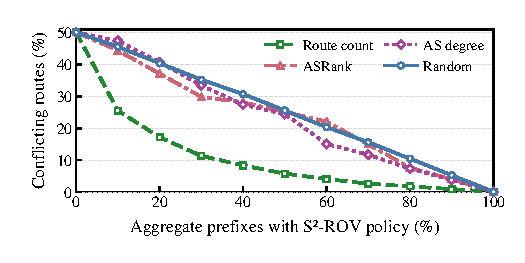
\includegraphics[width=\columnwidth,trim=0 10bp 0 0,clip]{figures/fig_openscope_placement}
\caption{Prioritizing aggregate prefixes for \ssrov{}.}
\label{fig:openscope-placement}
\end{figure}

When 20\% of aggregate prefixes have an \ssrov{} policy, the mean conflict rate is 17.2\% under Route count, against 37.1\% under ASRank, 40.7\% under AS degree, and 40.4\% under Random; at 50\% the rates are 5.8\%, 25.1\%, 24.4\%, and 25.6\%. Prioritizing by eligible observed routes therefore reduces conflicts faster than either AS-topology order on this route set.

\subsection{System Cost and Live Path Control}
\label{sec:eval-cost}

\emph{How do classification and policy update costs scale, and does an installed action persist through a relying party outage?} We replay controlled IPv4 and IPv6 policies and query sets through the reference engine of Section~\ref{sec:impl-engine}, using route and origin pairs from the 24 June 2026 RRC00 RIB~\cite{ripe-ris}. Each policy holds one marked base entry and zero or more noncovering ordinary entries at total sizes of 1, 64, 256, 1,024, and 4,096 records; the single-record condition holds only the marked base entry. Within each IP version the five conditions reuse the same 4,096 queries, which fall below the base marker and return \openscope{}.

Classification times the public classifier with state capture, including CIDR parsing, over 32 warm repeats in five fresh processes pinned to one Kunpeng 920 core under Python~3.12.3.

An update adds the marker to the base entry of an otherwise identical active policy: for each version and size the two immutable snapshots differ only in that marker bit, and timing covers deserialization with validation, canonicalization, and index construction, active replacement, and the fixed route's first \openscope{} classification over 20 fresh processes per cell.

\begin{figure}[tb]\centering
\subfloat[Classification throughput.]{%
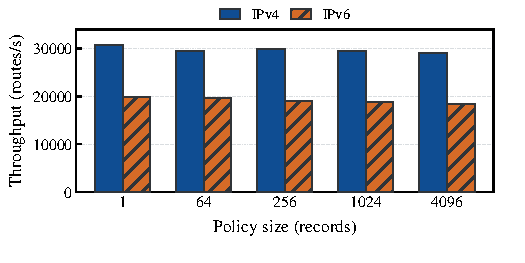
\includegraphics[width=0.85\columnwidth,trim=0 10bp 0 0,clip]{figures/fig_processing_cost_classify}%
\label{fig:processing-cost-classify}}\par
\subfloat[Update latency.]{%
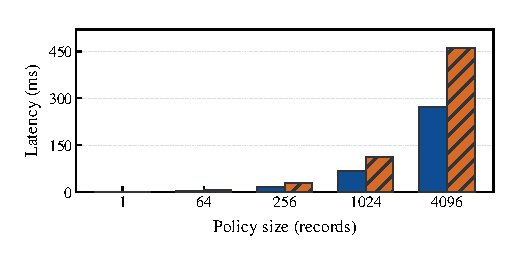
\includegraphics[width=0.85\columnwidth,trim=0 10bp 0 0,clip]{figures/fig_processing_cost_update}%
\label{fig:processing-cost-update}}
\subfigmaincaptionskip
\caption{System cost.}
\label{fig:system-cost}
\end{figure}

Classification throughput ranges from 29,149.8 to 30,647.4 routes/s for IPv4 and from 18,346.0 to 19,794.3 routes/s for IPv6 across the five sizes.

Figure~\ref{fig:system-cost}\subref{fig:processing-cost-update} reports update latency: it rises from 0.3 to 273.0\,ms for IPv4 and from 0.5 to 459.0\,ms for IPv6 across the same sizes, staying below 0.5\,s at 4,096 records. In the live path control, we interrupt the relying party for 15\,s after action installation, and the last installed action remains effective throughout the outage.

\subsection{Reachability and Origin Exposure}
\label{sec:eval-consequences}

\emph{How do intended route reachability and eligible unlisted origin exposure vary as more ASes are upgraded?} Deployment is the share of a fixed 589-AS upgrade set using \ssrov{} within a retained 77,429-AS BGPy graph~\cite{bgpy2023,gaorexford2001}. We evaluate 200 sampled aggregate-prefix cases in 10\% increments under five fixed upgrade orders; each pairs an aggregate with a proper subprefix originated by another AS. Section~\ref{sec:eval-conflict-reduction} instead varies ROA issuance and aggregate-prefix policy coverage.

The panels use different announcement sets and compare \ssrov{} with two conventional baselines: aggregate-only ROV, which uses only the aggregate ROA, and exact-match ROV, which lists the intended subprefix and its origin AS. Delivery is the percentage of the 77,429 topology ASes whose selected path ends at the plotted origin. \subref{fig:deployment-intended} reports intended-origin delivery; \subref{fig:deployment-competition} adds one eligible unlisted origin sampled uniformly per case and reports its delivery. \ssrov{} results average five fixed upgrade orders, and we report absolute percentages.

\begin{figure}[tb]\centering
\subfloat[Intended route delivery.]{%
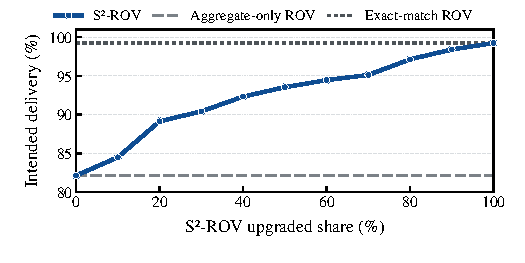
\includegraphics[width=0.95\columnwidth,trim=0 10bp 0 0,clip]{figures/fig_deployment_outcomes_a}%
\label{fig:deployment-intended}}\par
\subfloat[Unlisted origin delivery.]{%
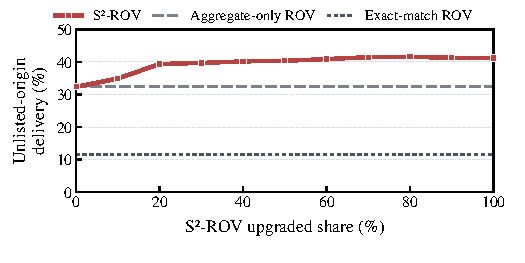
\includegraphics[width=0.95\columnwidth,trim=0 10bp 0 0,clip]{figures/fig_deployment_outcomes_b}%
\label{fig:deployment-competition}}
\subfigmaincaptionskip
\caption{Reachability and origin exposure.}
\label{fig:deployment-outcomes}
\end{figure}

At 50\% of the fixed upgrade set, \ssrov{} raises intended route delivery from 82.1\% under aggregate-only ROV to 93.5\%, while exact-match ROV reaches 99.2\%. In the competition setting it raises unlisted origin delivery from 32.4\% to 40.3\%; exact-match ROV yields 11.7\%.

When all 589 ASes in the set use \ssrov{}, intended route delivery reaches 99.2\%, matching exact-match ROV, while aggregate-only ROV remains at 82.1\%. Unlisted origin delivery rises from 32.4\% to 41.2\%, whereas exact-match ROV lowers it from 32.4\% to 11.7\%. The \ssrov{} value reaches 41.6\% at 80\% and declines to 41.2\% at 100\%.

A separate IPv6 candidate sensitivity evaluates the 0\%, 50\%, and 100\% endpoints for 21 distinct origin pairs from Table~\ref{tab:visibility-candidates}, yielding 210 scenarios across eight aggregate prefixes; at 100\%, every intended-only case matches the exact-match ROV reference. Relative to aggregate-only ROV, these eight aggregates gain 18.7 on average in intended delivery and 17.6 in unlisted-origin exposure in the separate competition setting, while the median change across pairs is 0.0 and 14.0.

\subsection{Attack Reachability}
\label{sec:eval-security}

{\revstart \emph{What does a marked region admit to an adversary?} We reuse the routing model of Section~\ref{sec:eval-consequences} and add a same-length sibling prefix announced by the adversary: the other child of the leaf's supernet at the leaf's prefix length. Conventional authorization remains one aggregate ROA for the aggregate origin with \texttt{maxLength} equal to the aggregate length; the treatment configures an \ssrov{} policy for all 589 ASes in the upgrade set and maps \openscope{} to acceptance. Each of the 200 sampled units runs in both cells, giving 600 trials under the same stratification and weights.}

{\revstart Within the 589 upgrading ASes, the adversary's sibling route is selected by 0.0\% of them under conventional ROV and by 98.6\% once every AS in the set runs \ssrov{}. Across all 77,429 modeled ASes reachability rises from 51.7\% to 98.2\%; the conventional value is not zero because ASes outside the upgrade set do not filter. Destination-level attribution to the adversary rises from 68.0\% to 98.2\%. This is the measured cost of the state: inside a marked region the upgrade set no longer separates the adversary from the intended origin, and only the local action does.}

{\revstart \emph{How much does the local action matter?} The routing model applies one admission decision per state, so these outcomes correspond to accepting \openscope{}. Rejecting it reproduces the aggregate-only ROV outcomes by construction, since an \openscope{} route is one that no ROA matches: 82.1\% intended delivery and 32.4\% unlisted-origin delivery. The two measured endpoints therefore bracket the action spectrum at the level of admission. A preference between them would matter only where an \openscope{} route competes for the same prefix with an \explicit{} route from a different origin, which neither announcement set here produces; the prototype assigns LP~300 to \explicit{} and LP~200 to \openscope{}, so a matching ROA wins once it exists.}

{\revstart \emph{Scope of these counts.} All 589 pairs in the conflict replay are covered by at least one ROA, so \notfound{} does not enter that estimand; the classifier leaves \notfound{} unchanged, whereas withdrawing the covering entry would move a route to \notfound{} while also withdrawing the aggregate's \explicit{} evidence (Case~2 of Figure~\ref{fig:motivation}). Both reported baselines are therefore ROV configurations rather than a no-RPKI arm.}
